\section{Introduction}
\label{sec:introduction}

\todo{rewrite a little... sections are directly copy and pasted from the old document.}
The deployment of the ArgonCube 2x2 Demonstrator in the MINOS-ND hall as the core component of ProtoDUNE-ND, a neutrino engineering testbench for the DUNE near detector (ND) has been presented in Ref.~\cite{2x2@FNAL}. The ArgonCube 2x2 Demonstrator will serve as an engineering test-stand for developing the techniques required to deploy a full-scale version of ArgonCube in the DUNE ND. This provides an essential opportunity to characterize the novel ArgonCube readout technologies response, and develop the reconstruction tools necessary for operating ArgonCube in the DUNE ND.

However, given the 2x2's size and the relatively high energy NuMI ME beam, many events will not be contained in the 2x2 alone. Figure~\ref{fig:leaky_event} shows a neutral current event where many pions are produced, but in which the pions and subsequent hadronic showers extend far beyond the detector. Indeed, many such events would not be contained in the full ArgonCube deployment at the DUNE ND, in the LBNF beamline, and for charged-current events, the muon will be uncontained most of the time. For this reason, and because it is not possible to magnetize the large LAr component, further, magnetized, tracking detectors are proposed downstream of ArgonCube in the full DUNE ND complex, and the requirement to tag side-escaping particles is discussed in Ref.~\cite{dune_ndcsg}. Two additional subdetector options are being considered for the DUNE-ND design, in addition to ArgonCube~\cite{dune_ndcsg}: the Three-Dimensional Scintillator Tracking (3DST) detector; and a magnetized high pressure argon-gas TPC (HPgTPC).

\begin{figure}[htb]
	\centering
	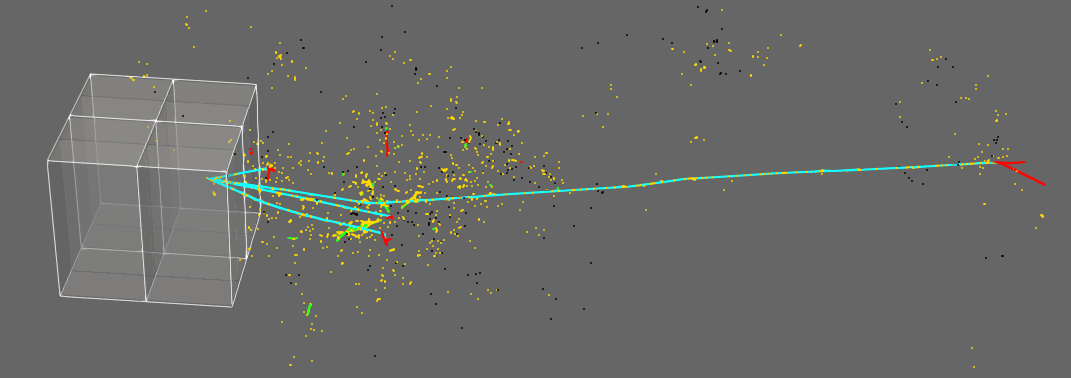
\includegraphics[width=0.8\textwidth]{{plots/EventDisplays/8.17GeV_rectangle_crop}.png}
	\caption{Example ArgonBox simulated event for an 8.17 GeV $\nu_{\mu}$--argon neutral-current multi-pion interaction, in which the pions are not contained in the module. Energy deposits in a bulk volume of LAr are color-coded according to the particle type: $\pi^{\pm}$ --- blue; $\mu^{\pm}$ --- purple; $e^{+}$ --- green; $e^{-}$ --- yellow; proton --- red; recoiling nuclei --- black. The event vertex was randomly placed inside the active volume of the ArgonCube 2x2 Demonstrator, the geometry for which is superimposed on these images, but which is not simulated by ArgonBox. Taken from Ref.~\cite{2x2@FNAL}}
	\label{fig:leaky_event}
\end{figure}

Ref.~\cite{2x2@FNAL} notes that although the detector physics case for the ArgonCube 2x2 alone is compelling, a large fraction of the high energy on-axis NuMI medium energy (ME) beam would not be fully contained in the ArgonCube 2x2 Demonstrator alone, and a number of further, or extended, detector physics studies would be possible if and when additional subdetector prototypes are introduced to ProtoDUNE-ND. Prototypes for these detectors are currently being planned, and the ProtoDUNE-ND complex is intended to evolve over time to accommodate them. The cryogenic system for the ArgonCube 2x2 will be moveable to test key components of the DUNE-PRISM technical design, which will allow ProtoDUNE-ND to be easily reconfigured to accommodate any future prototype detectors. In the absence of prototypes for the HPgTPC or 3DST on a comparable scale as the 2x2, on the timeline of initial ProtoDUNE-ND operations in October 2020, in this document, we propose the ProtoDUNE-ND-Tracker, which uses repurposed MINERvA and MINOS-ND hardware, already on-axis in the NuMI medium energy (ME) beam, to provide a low cost tracking detector to enhance the detector physics reach of ProtoDUNE-ND, following the decommissioning of MINERvA in Summer 2019. This document is based on discussions with members of MINERvA and other active DUNE ND collaborators who have expressed an interest in joining the ProtoDUNE-ND effort.

%check this after full read through
As well as expanding the phase-space of fully contained events, the proposed ProtoDUNE-ND-Tracker provides a functionally very similar detector to the fast scintillator detector components included in all potential DUNE ND configurations identified in Ref.~\cite{dune_ndcsg}. The ability to reconstruct tracks between a fast scintillator detector, and both liquid and gaseous argon TPCs, with a slow charge readout, but fast light readout, is a keystone of the future DUNE ND reconstruction. Studies pairing the 2x2 with components of MINERvA are presented in Section~\ref{sec:MINERvA}, including a discussion on track matching between fast and slow detectors and studies of acceptance and neutron tagging. Discussion of how MINOS-ND could be repurposed to provide a valuable further reference for calibrating the ProtoDUNE-ND response as a function of momentum is discussed in Section~\ref{sec:MINOS}. A cost estimate for the operation of the MINERvA components and method of reducing the running cost of MINOS is presented in Section~\ref{sec:costs}. Conclusions are presented in Section~\ref{sec:conclusions}.

% We note that clearly, the scientific benefit in having a downstream tracker included in ProtoDUNE-ND, or repurposing an existing tracker, must be evaluated against the technical feasibility and the availability of resources (person power and financial). These costs would have to be shared between ProtoDUNE-ND collaborators and Fermilab. 
